\section*{Side-Chain Entropy in Naturally Occurring Proteins}
\label{sec:side_chain_entropy_of_x_ray_structures}
In holding with a classic scientific tradition, we can listen to nature and learn what she has to tell us. In this case, that means gathering information about naturally occurring proteins and subjecting this information to analytical techniques that might reveal something about the role of side-chain entropy. This can be an especially fruitful line of investigation when it comes to aspects of proteins simply because nature has a vastly larger laboratory than any man could create and experiments have been on-going for literally billions of years. All we have to do is frame our question in such a way that evolution will have already provided an answer.

One way we can do that is to ask a question about protein stability. Our interest is in the forces that give shape to a protein structure, but it's been well established that protein structures are marginally stable. In order to increase the stability of these structures, the forces favoring a native protein structure will need to be strengthened. To find which forces are important, we need only look at which forces have increased in magnitude in an environment where protein stability is key. Luckily, hyperthermophilic bacteria thrive in exactly that sort of an environment.

This is the technique adopted by Berezovsky, \emph{et al.}\cite{Berezovsky:2005p40} in comparing protein sequences from mesophilic and thermophilic bacteria and looking at their amino acid content and side-chain entropy. They begin with an interesting simplification of a protein model commonly known as the $\mathrm{G\bar{o}}$ model. This model simplifies the calculation of potential energy by only considering amino acid interactions present in the native state. While this might seem like a rather drastic simplification, it allows the experimenter to focus on features of the amino acid backbone and side-chains. In other words, they sacrifice detail in the folding pathway, but are able to retain atomic detail of the structure.

Using the number of accessible rotameric states as a measure of side-chain entropy, the first observation this group makes is that, in folded state of hydrolase H from both \emph{Escherichia coli} and \emph{Thermus thermophilus}, lysine retains more of its side-chain entropy than arginine (an average of 20.1 vs 3.5 accessible rotamers per residue, respectively, in the folded state). This is mildly surprising as both lysine and arginine have similar chemical properties, they are both positively charged, and the both have the same total number of rotamers. The difference between the two stems from the guanadinium group of arginine, which is bulky and restricts its motion in the core of the protein structure.

Next, they expanded their investigation to 18 pairs of proteins from \emph{E. coli} and \emph{T. thermophilus}. This time, instead of simply looking at absolute numbers of rotamers, they carried out Monte Carlo unfolding simulations and compared the number of observed rotamers in the folded and unfolded states for lysine and arginine (Figure~\ref{fig:rotamer_ratios}). Consistent with their initial findings, the lysines have a much smaller discrepancy between the observed rotamers in the folded and unfolded states than the arginines.

\begin{figure}[h]
	\center
	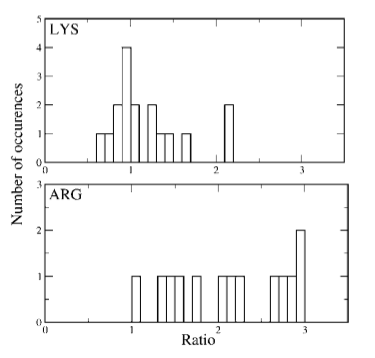
\includegraphics{rotamer_ratio}
	\caption{(Borrowed from \cite{Berezovsky:2005p40}) Distribution of the Ratios of the Number of Rotamers in Unfolded and Folded States in a Representative Set of Proteins.}
	\label{fig:rotamer_ratios}
\end{figure}

From these observations, they form a hypothesis that replacing arginines with lysines in the hydrolase H from \emph{E. coli} will increase its temperature stability. There are a few difficulties with this sort of experiment. First, switching out residues like this without making corresponding changes to other interacting residues will decrease the number of favorable interactions in the native state. Second, even using the $\mathrm{G\bar{o}}$ model approximations, it is still difficult to collect enough Monte Carlo samples to definitively say if switching lysine for arginine has a stabilizing effect. Their results seem to indicate that this is the case but are far from convincing.

In addition to attempting to model their hypothesis, Berezovsky, \emph{et al.} look to the available proteomes of 38 mesophilic and 12 hyperthermophilic bacteria. Here, they find that the arginine content of the hyperthermophiles is less than that of the mesopiles, and correspondingly, the hyperthermopilic lysine content is greater (Figure~\ref{fig:aa_content}). Looking at the underlying genomic sequences for each proteome, they were able to rule out the possibility of this being an artifact of DNA-base bias in all but two cases.

\begin{figure}[h]
	\center
	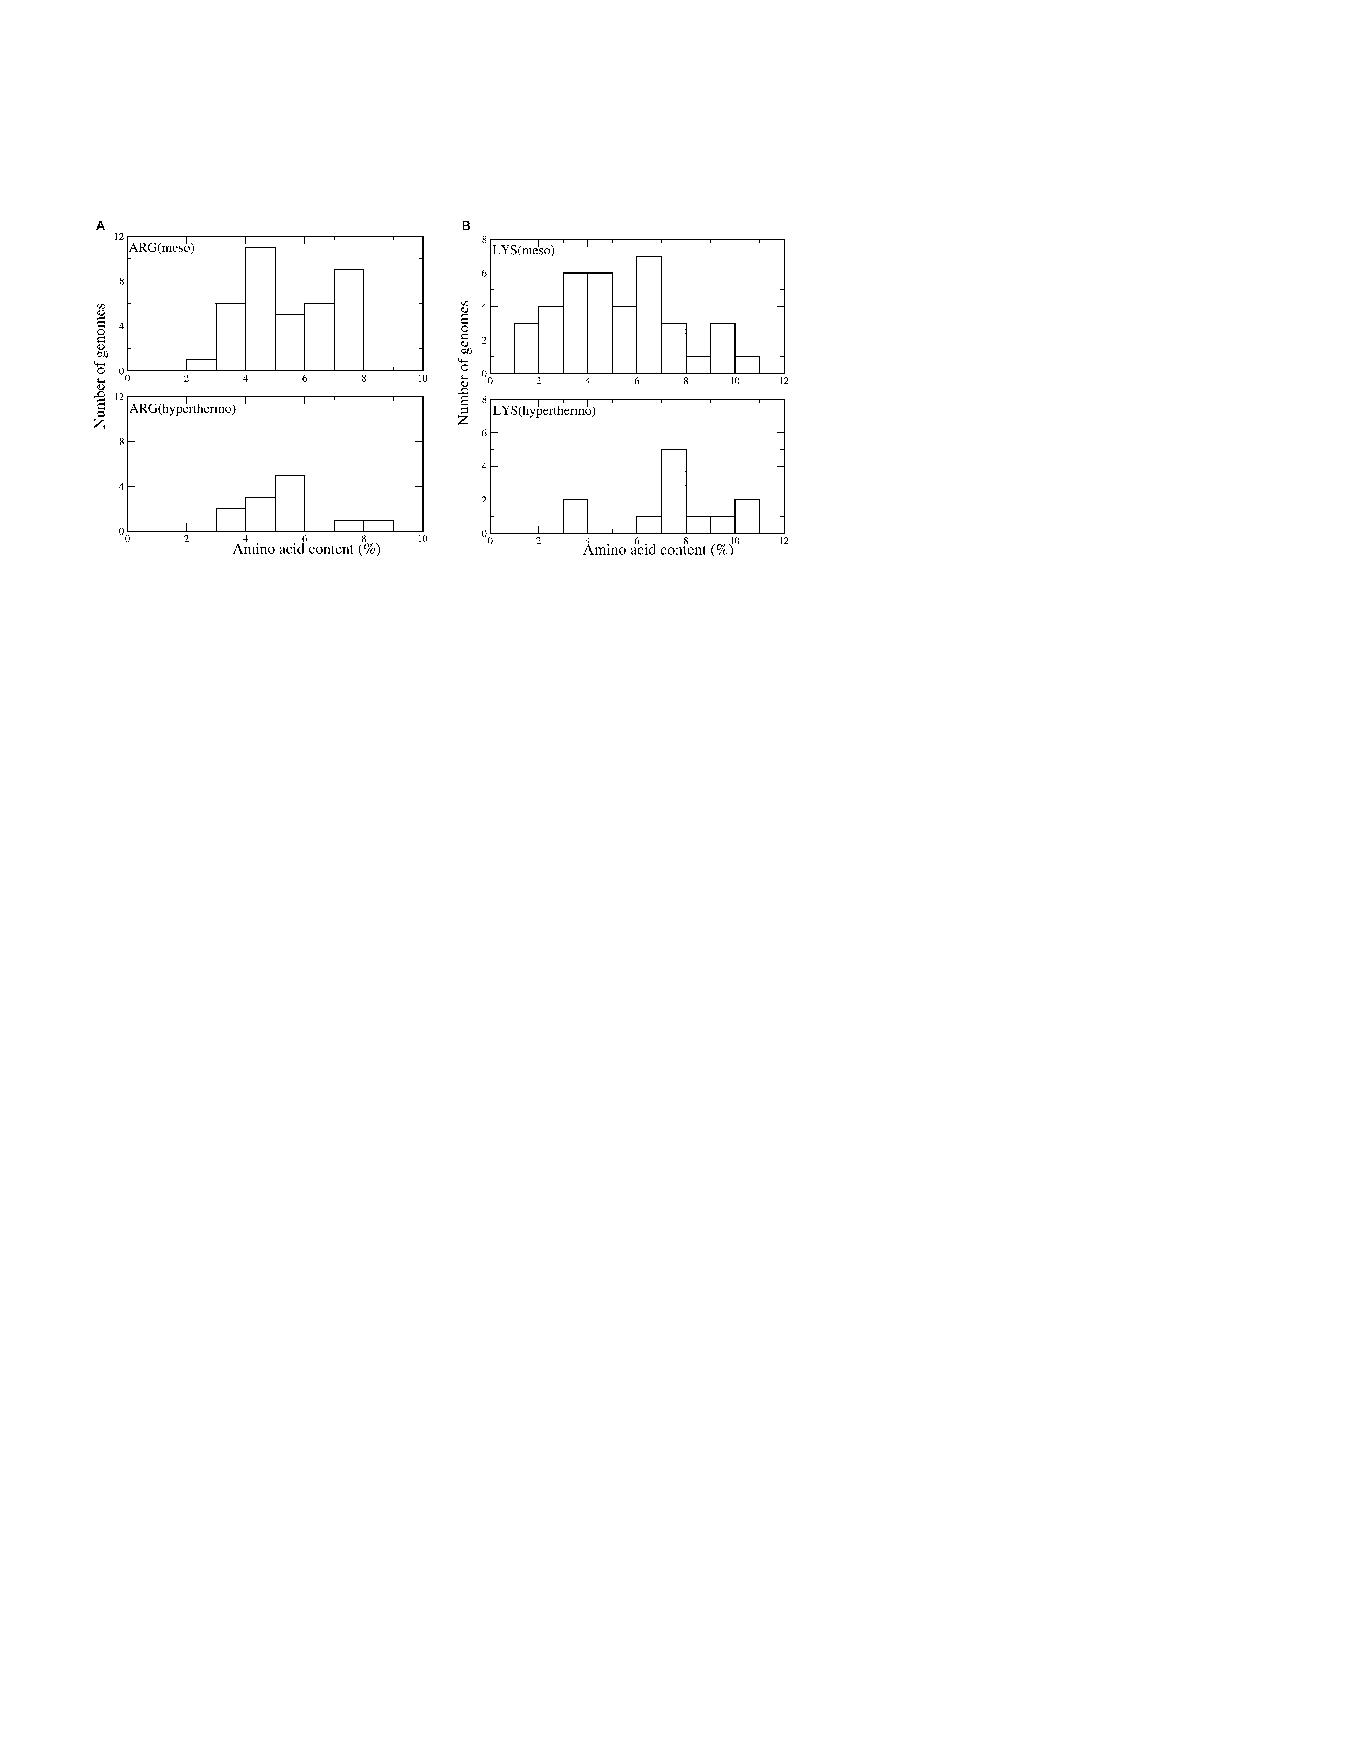
\includegraphics{aa_content}
	\caption{(Borrowed from \cite{Berezovsky:2005p40}) Histograms of the Content of Charged Amino Acid Residues in Hyperthermophilic Genomes Compared with Mesophilic Genomes. (A) Arginine content of mesophilic genomes, top, and hyperthermophile genomes, bottom. (B) Lysine content of mesophilic genomes, top, and hyperthermophile genomes, bottom. }
	\label{fig:aa_content}
\end{figure}

Instead of looking for clues in protein sequences, Zhang and Liu\cite{Zhang:2006p11} decided to look to protein structures. They use a variation on a Sequential Monte Carlo method to approximate, from a set of experimentally determined protein structures, the entropy resulting from side-chain motions. Their initial results using this technique show that side-chain entropy increases linearly with chain length, and that as chains grow beyond a threshold length, the buried residues in a structure contribute about half of the total side-chain entropy for a protein. Both of these results are consistent with what is already known of side-chain entropy.

As a next step, they calculated the side-chain entropy of 24 distinct proteins and a corresponding set of decoy protein structures. The logic here is that, if side-chain entropy is important, then it should be useful as a metric to discriminate between the real and the decoy proteins. What they found was very convincing. If they plotted the side-chain entropy versus the radius of gyration, a measure of compactness, then in half of the cases studied the real structure had a clearly greater side-chain entropy than for any of the structures of similar compactness. In the half where this was not the case, there were extra constraints which led to the native structure having a lower entropy. Even for dimeric proteins, they were able to plot side-chain entropy versus the number of interfacial contacts and found that the native structures were convincing outliers.

\begin{itemize}
	\item X-ray vs NMR
	\item Scoring
	\item wrap-it-up...
\end{itemize}

\begin{figure}[h]
	\center
	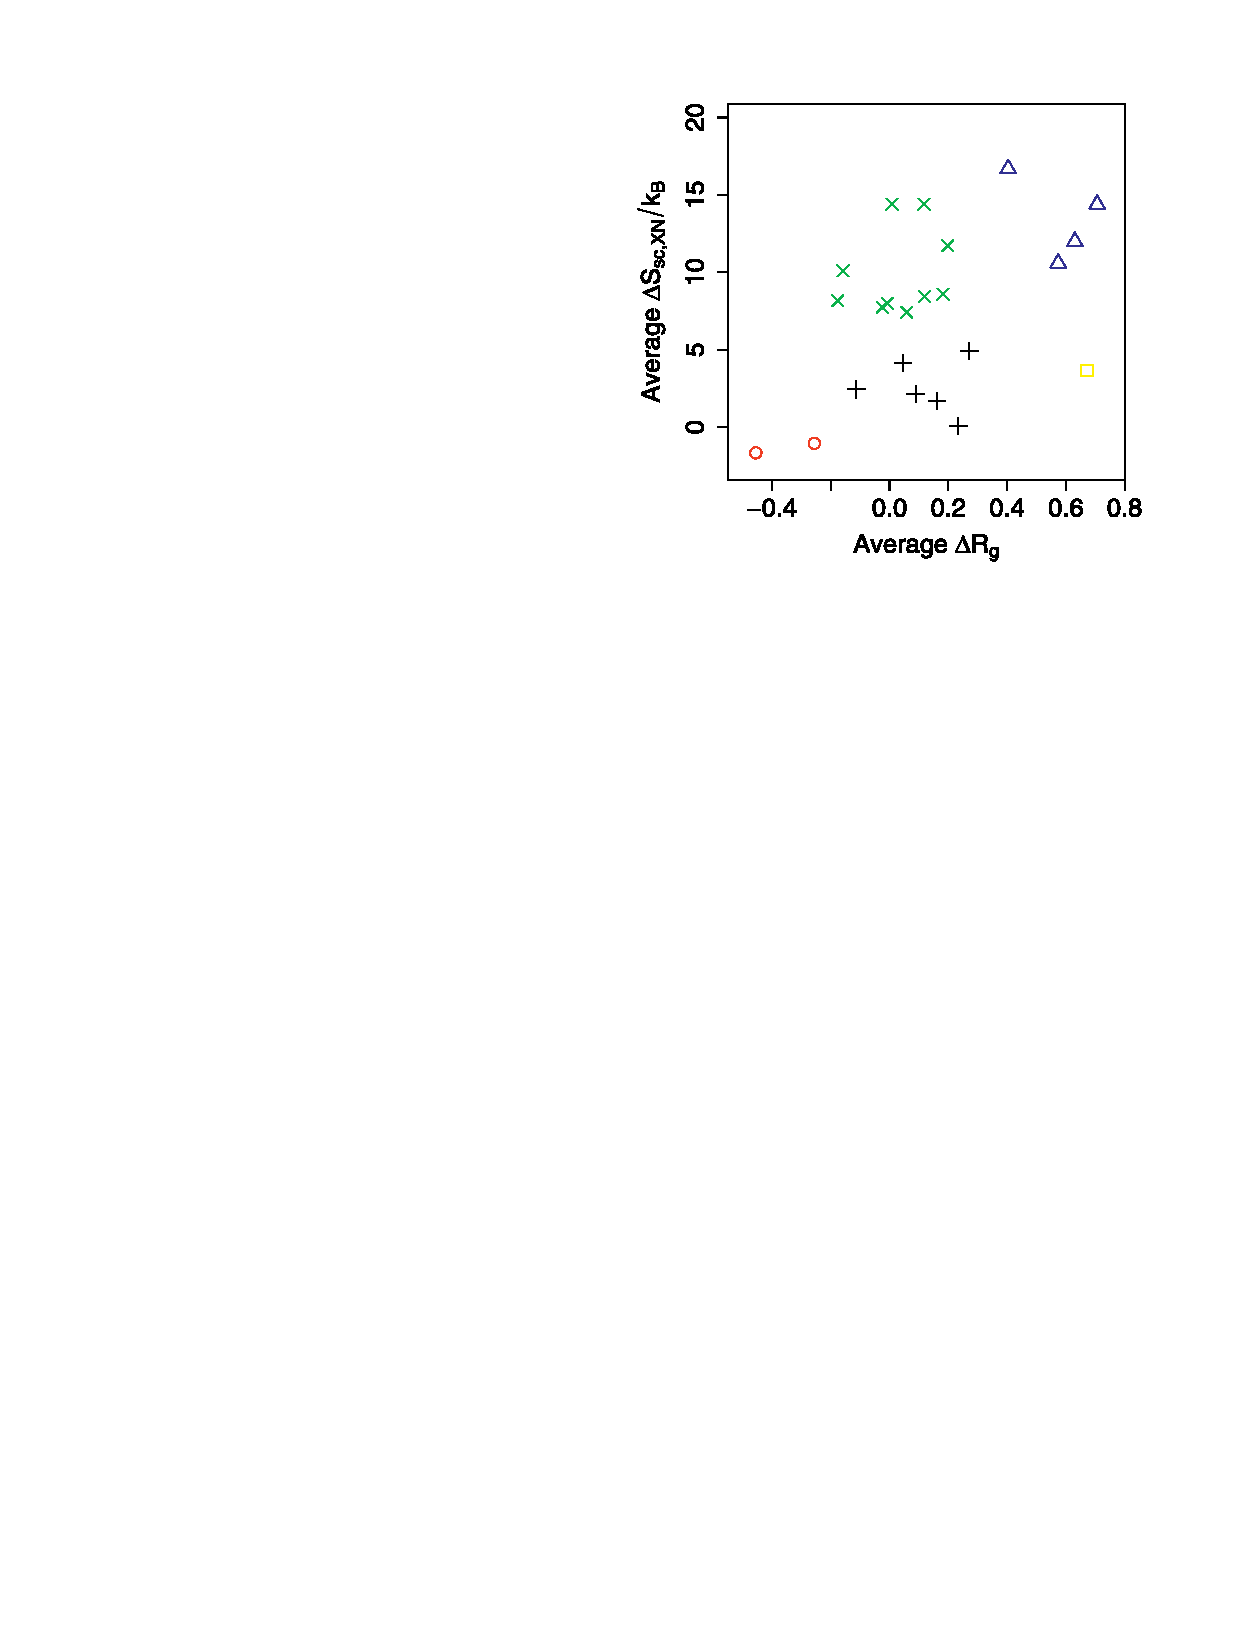
\includegraphics{deltaS_descrimination}
	\caption{(Borrowed from \cite{Zhang:2006p11}) Side-Chain Entropy of NMR and X-Ray Structures vs $R_g$. `X's are proteins whose X-ray structures have much higher side-chain entropy than but similar $R_g$ to the corresponding NMR structures. Triangles are proteins whose X-ray structures gain considerable side-chain entropy by packing a little looser. Circles are proteins whose X-ray structures pack tighter than NMR structures but with comparable side-chain entropy. `+'s are small proteins with both small $R_g$ and $\Delta S_{XN}$.}
	\label{fig:deltaS_descrimination}
\end{figure}